% Chapter discussion

\chapter{Materials and Methods(5-10 pagine} % Main chapter title

\label{Chapter7} % For referencing the chapter elsewhere, use \ref{Chapter7} 

%----------------------------------------------------------------------------------------
% Define some commands to keep the formatting separated from the content 
porta le metodiche utilizzate per lo svolgimento degli esperimenti descritti nella sezione “Risultati ottenuti dal candidato”.

%chiedere ad Enza, se per seqgen metto albero

\section{Bubblepop} 
\subsection{Odgi}

I built the \textit{bubblepop} function utilizing the odgi library(\cite{eizenga2020succinct})\\

odgi (Optimized Dynamic Graph Implementation) is based on a node centric encoding of the graph that is designed to improve cache coherency when traversing or modifying the graph. This encoding is split between graph topology and paths, which is important for achieving a good balance of run time performance and memory usage on real-world graphs with large path sets. Each node’s sequence and edges are encoded in a byte array using a variable-length integer encoding scheme. Edges are described in terms of a relative offset between the rank of this node in the sorted array of nodes of the graph and the node to which the edge arrives.

The first step is convert the graph in GFA format in a graph in odgi format with:

\begin{verbatim}
odgi build -g graph.gfa -o graph.og
\end{verbatim}

Before executing any of the following commands, initialize the graph object with:

\begin{verbatim}
g=odgi.graph()
\end{verbatim}

Start this function after load GFA, with use two recursive algorithms. 

\subsection{DFS}
Depth first Search is a recursive algorithm for searching all the vertices of a graph or tree data structure.
The DFS algorithm works as follows:

\begin{verbatim}

def dfs(graph, start, visited=None):
    if visited is None:
        visited = set()
    visited.add(start)
    print(start)
    for next in graph[start] - visited:
        dfs(graph, next, visited)
    return visited

\end{verbatim}

\subsection{BFS}
Breadth first Search is a recursive algorithm for searching all the vertices of a tree data structure.
This algorithm works as follows:

\begin{verbatim}
def bfs(graph, root): 
    visited, queue = set(), collections.deque([root])
    visited.add(root)
    while queue: 
        vertex = queue.popleft()
        for neighbour in graph[vertex]: 
            if neighbour not in visited: 
                visited.add(neighbour) 
                queue.append(neighbour) 
\end{verbatim}

I implement this algoritm that is availabe on the git repository of the project (\url{}) 

%citare: https://www.programiz.com/dsa/graph-bfs 

\subsection{BubblesCalling}

After BFS I continue with a key point of a code, dictionary that identify start and end of bubbles Fig:({\ref{fig:bubblepop.png}}).\\

For define start and end, I calculate distance of node in the three obtained with BFS from root, the chose of root is arbitrary. I use two lists: distance from root and ordinary nodes with the same distance.
Key of a dictionary represent distance and value nodes with the same distance. 

\begin{verbatim}
    
dist_to_num_nodes = dict()   
for node_id, distance in distances_dict.items():
    if distance not in dist_to_num_nodes.keys():   
        dist_to_num_nodes[distance] = 0
    dist_to_num_nodes[distance] += 1

\end{verbatim}

\section{gfa2vcf}

Before run the script GfatoVcf.py, you need to:

1. Convert the GFA format to the ODGI format because this is the format taken as input to the script.
2. With -path specify the path of the odgi library and with -input specify the input file as odgi format

\begin{verbatim}
 python GfatoVcf.py -path /../odgi/lib/ -input /../input.odgi   
\end{verbatim}
    
This code start with the dictionary that there is in \textit{bubblepop}, I continue to identify SNV and INDEL.
\subsection{Extracting Variant and VCF}

\begin{itemize}
\item Chose path as REF: I chose a path (or paths) from the beginning by recording sequences, it is corresponds to REF. Sequence not present in REF, the center of bubble is ALT.

%mettere codice? tipo questo esempio
%if current_node_id_ref == current_node_id_path:
                    
                    %node_seq = g.get_sequence(g.get_handle(current_node_id_ref))
                    %pos_ref += len(node_seq)
                    %pos_path = pos_ref

                    %current_index_step_ref += 1
                    %current_index_step_path += 1
                %else:
                    %succ_node_id_path = path[current_index_step_path + 1]
                    %succ_node_id_ref = ref_path[current_index_step_ref + start_node_index_in_ref_path + 1]
                    %if succ_node_id_ref == current_node_id_path:
                    %print(DEL)
                    
\item Deletion in VCF: If the succ node in the (path that I chose as REF) REF is the current node in the current path, it means that in the current path a node is missing, so there is a DELETION respect to the reference.

\item Insertion in VCF: If the succ node in the current path there is a node in the REF, it means that in the current path there is a node that is missing in the REF, that is an INSERTION.

\item SNV in VCF: Else if sequence is different from the same node in REF and ALT, it is a SNV.

\item POS in VCF: Length of sequence in a node corresponds to POS.
POS, for example (NODE1 ATG)POS is 3 (length of sequence); for (NODE2 AT) POS is 5 because is the sum of the length of the previous node sequence plus the current node length sequence.   
\end{itemize}


\begin{figure}[H]
\centering
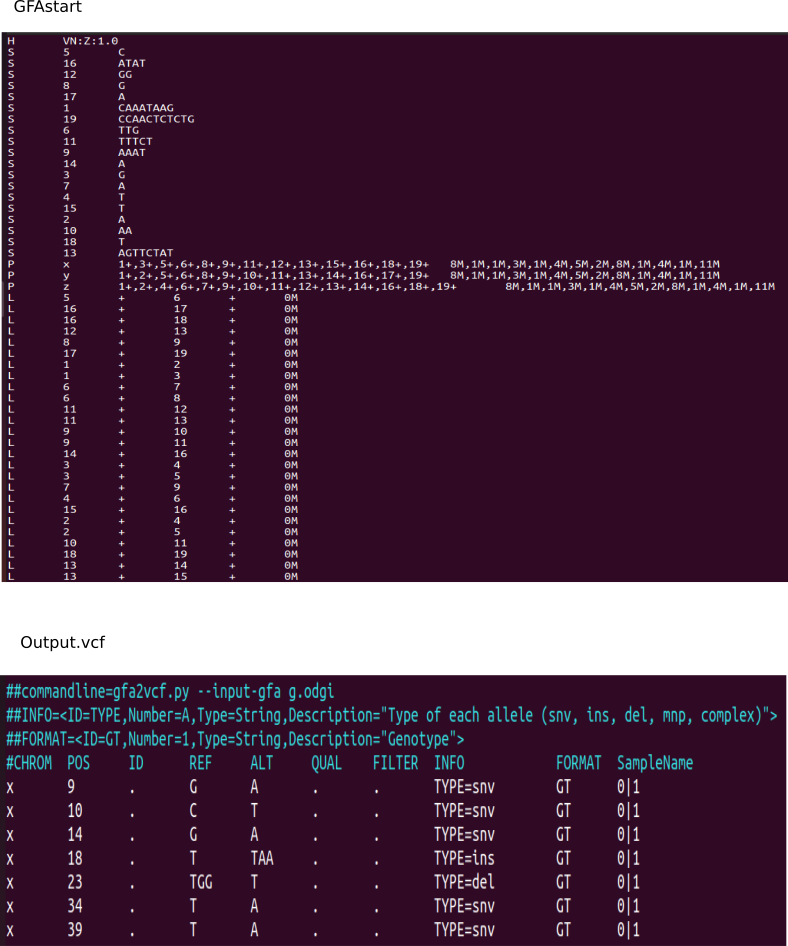
\includegraphics[width=0.70 \textwidth]{fig/gfa2vcf.png}
\decoRule
\caption{\textit{GFAstart to VCF} transforms a GFAstart in VCF}
\label{fig:validationgraph.png}
\end{figure}
\subsection{Validation VCF}

I use vg tools for working with genome variation graphs for validate VCF obtained from GFA. 

VCF files generated by \textit{gfa2vcf} is compressed and indexed. Compression optimizes files storage and transfer. Indexing allows fast access to large files. 
\begin{itemize}
\item Compress and indexing
\end{itemize}

Compression was done using Bgzip (\url{https://www.htslib.org/doc/bgzip.html#DESCRIPTION}) that "compresses files into a series of small (less than 64K) 'BGZF' blocks. This allows indexes to be built against the compressed file and used to retrieve portions of the data without having to decompress the entire file"

\begin{verbatim}
~/bin/bgzip output.vcf > output.vcf.gz
\end{verbatim}

Indexing was done using Tabix (\url{https://www.htslib.org/doc/tabix.html}) that "indexes a TAB-delimited genome position file in.tab.bgz and creates an index file". 
The command line takes in input the compressed file from BGZIP and produces an indexed file: 

\begin{verbatim}
~tabix -h output.vcf.gz  
\end{verbatim}

\begin{itemize}
\item  vg construct and view
\end{itemize}
I use indexed file as input of vg construct with reference that I chose. For obtained this output represent in Fig: ( \ref{fig:validationgraph.png} B). I use vgview.

\begin{verbatim}
vg construct -v output.vcf.gz -r reference.fa > VcftoGraph.vg

vg view -dp VcftoGraph.vg | dot -Tpdf -o ValidationGraph.pdf


\end{verbatim}

\section{bcftools and vcftools}

With seqgen2gfa+vcf, I'm starting with Seq-Gen and I obtained GFAformat and VCFformat. 

For calculate allele frequencies on VCF that I obtained from Seq-Gen I use bcftools and vcftools.

\begin{itemize}
    \item Bgzip and Tabix for each replicates

\begin{verbatim}
for f in ./*.vcf; do bgzip "$f"; done   
for f in ./*.vcf.gz; do tabix -h "$f"; done
\end{verbatim}



\item bcftools

Extracting individuals of two populations was done using bcftools (\url{http://samtools.github.io/bcftools/bcftools.html#view})  is a set of utilities that manipulate variant calls in the Variant Call Format (VCF) and its binary counterpart BCF.  I extract individuals with view " subset and filter VCF or BCF files by position and filtering expression".


\begin{verbatim}
parallel bcftools view -S pop_1.txt seqgen_rep{1}.vcf.gz
-o seqgen_rep{1}.pop1.bcf.vcf.gz ::: {1..100} 

parallel bcftools view -S pop_2.txt seqgen_rep{1}.vcf.gz 
-o seqgen_rep{1}.pop2.bcf.vcf ::: {1..100}  
\end{verbatim}

\item vcftools

Calculate allele frequencies from two populations was done using vcftools (\url{http://http://vcftools.sourceforge.net/man_latest.html}), vcftools is a suite of functions for use on genetic variation data in the form of VCF and BCF files. The tools provided will be used mainly to summarize data, run calculations on data, filter out data, and convert data into other useful file formats.

\begin{verbatim}
parallel vcftools --gzvcf seqgen_rep{1}.pop1.bcf.vcf.gz 
--freq --out ms_rep{1}.bcf.pop1.vcf ::: {1..100} 

parallel vcftools  --gzvcf seqgen_rep{1}.pop2.bcf.vcf.gz --freq 
--out ms_rep{1}.bcf.pop2.vcf ::: {1..100}  
\end{verbatim}


%calculate fst, with script fstonvcf

\end{itemize}


\section{Visualization results of Fst from GFA and VCF}

I use R for visualitazion of Fst \ref{fig:fsttime.png}

Import t1,t2,t3 i.e three time of separation of two populations.

\begin{verbatim}

w <- as.data.frame(rbind(t1, t2, t3))
w$time <- c("T1", "T2", "T3")
myd <-w %>% gather(fst, obs, V1:V100)
myd$type<-"from_VCF"

q <- as.data.frame(rbind(t1, t2, t3))
q$time <- c("T1", "T2", "T3")
myd2 <-q %>% gather(fst, obs, V1:V92)

myd2$type<-"from_GFA"

final<-rbind(myd, myd2)

ggplot(final, aes(obs, color=time, linetype=type)) + geom_density() + xlab("FST") + ggtitle("FST distributions from 100 replicates") +scale_color_manual(values=c("#fe346e", "#ffbd69", "#381460"))

 ggsave("fst_time.png", width = 25, height = 15, units = "cm")
 
\end{verbatim}

\section{pangenome HLA}

I will use tools supporting the variation graph data model, as described at the pangenome tools (\url{https://pangenome.github.io/}), to build pangenome data from HLA genomes.\\

I start with 9 sequences from chr6 Homo Sapiens, downloads its in formato fasta file. 


\item minimap 
I use (\url{https://lh3.github.io/minimap2/minimap2.html}), is a fast sequence mapping and alignment program that can find overlaps between long noisy reads, or map long reads or their assemblies to a reference genome optionally with detailed alignment. 

I use minimap and I obtained paf format file and bgzip it.

\begin{verbatim}
minimap2 -t 16 -c -X $f $f |gzip > HLA/$b.paf.gz 
\end{verbatim}


\item seqwish and fpa
The alignment to variation graph inducer seqwish \url{https://github.com/ekg/seqwish} renders a set of sequences and alignments into the equivalent variation graph.
Seqwish supports minimap2's PAF format output.
With fpa (filtrare allineamenti sotto 3kb)
    
\begin{verbatim}
seqwish -s HLA/$b.fa.gz -p <(zcat HLA/$b.paf.gz fpa drop -l 2000) -g HLA-gfas/$b.gfa -P
\end{verbatim}
  
\item odgi
With odgi build command constructs a succinct variation graph from a GFA. Currently, only GFA1 is supported.


With odgi sorts a succinct variation graph, sort for have a sort visualization.


With odgi viz I visualize pangenome and save ordinate pangenome. 

\begin{verbatim}
odgi build -g HLA-gfas/$b.gfa -o - | odgi sort -i - -o - -p Ygs -t 16 -P > HLA-gfas/$b.sort.odgi 
odgi viz -i HLA-gfas/$b.sort.odgi -o HLA-gfas/$b.sort.odgi.png -x 4000 -y 500 -R
odgi view -i HLA-gfas/$b.sort.odgi -g > HLA-gfas/$b.sort.gfa
\end{verbatim}

\item VCF and Allelefrequencies

I applicate \textit{gfa2vcf} and I obtained VCF.

\begin{verbatim}
GfatoVcf.py -input E-3133.og -path odgi
\end{verbatim}

For validate this result I use vg.

\begin{verbatim}
vg view -Fv E-3133.gfa > E-3133.vg
vg index E-3133.vg -x E-3133.xg
vg deconstruct -p "gi|568815592:30489405-30494204" E-3133.xg 
\end{verbatim}

I obtained the same result. 

For visualize (\ref{fig:pangenome.png}) I use this commands:

\begin{verbatim}
odgi sort -i E-3133.og  -o - | odgi viz -i - -o E-3133.sorted.png -x 15000
\end{verbatim}


  


